\documentclass[11pt]{article}
\usepackage{amsmath,amssymb,booktabs,graphicx,hyperref,tabularx}
\usepackage[margin=1in]{geometry}
\hypersetup{colorlinks=true,linkcolor=blue,citecolor=blue,urlcolor=blue}
\newcommand{\rhoA}{\rho_{\mathrm{A}}}
\newcommand{\epsPl}{\varepsilon_{\mathrm{Pl}}}
\newcommand{\rhoPl}{\rho_{\mathrm{Pl}}}
\title{The Einstein--Cartan Spin-Density Bound in Three Normalisations}
\author{William Alexander Aldred\\ Aldred Industries, Davison, Michigan, USA}
\date{19 November 2026\\ Revision 5, fourth revision --- research draft, not peer reviewed}
\begin{document}
\maketitle

\begin{abstract}
I compute the spin-density bound of Einstein--Cartan gravity in three
normalisations: the density at which the spin-torsion term cancels the
mass-energy density of a neutron gas, so that the effective density
vanishes and a collapsing homogeneous dust cloud turns around instead of
reaching a singularity. The bound is the Kopczy\'nski--Trautman bound of
1972--73, and I claim no priority for it. The calculation depends on one
prescription: how the spin-squared average of an unpolarised
spin-$\tfrac12$ gas is taken. I adopt the classical spin-fluid value,
which gives $\rhoA = 3.8871\times10^{55}\ \mathrm{g\,cm^{-3}}$ for
neutrons, as a stated choice on grounds of sourcing and consistency ---
the factor of four between it and the literature value,
$\rhoA = 9.7178\times10^{54}\ \mathrm{g\,cm^{-3}}$, is unresolved, and
the literature value is carried beside it at every step. A
preliminary normal-ordered calculation, reported in the house files and
not deposited with this paper, gives a negative spin-squared sign that
would remove the bounce entirely; the full covariant Wigner-function
evaluation that would settle the sign has not been done.
With the full relativistic Fermi-gas energy density the balance moves to
$20.25\,\epsPl$ on the adopted normalisation and $1.27\,\epsPl$ on the
literature one: the bounce sits at or above the Planck density, outside
the demonstrated validity of classical Einstein--Cartan theory. The flat
Friedmann bounce is demonstrated on the dust model; a black-hole interior bounce, a baby
universe, and a rotating-progenitor signature are not. The galaxy-spin
axis test is inconclusive. The vacuum-count check passes its tolerance
rule on one combination only --- the adopted normalisation on the
measured bench, $N^* = 281.775 \pm 0.026$, $0.225$ bits from the target
--- and fails on the literature normalisation and on the earlier papers'
own density, where the 282-cell count undershoots the measured density
by about $36\%$; the count is not derived. Every number in Tables 1--4
is recomputed from CODATA 2018 constants \cite{CODATA18} by a script
that runs from the deposited files alone; the observational numbers in
\S7 are not covered by that script.
\end{abstract}

\section{Introduction}

Einstein--Cartan gravity adds one thing to general relativity: spacetime
has torsion, and the torsion is fixed algebraically by the spin of
matter. Eliminate the torsion from the field equations and the spin
appears as a correction to the energy density, quadratic in the spin
density and negative in sign. At high enough density the correction wins
over the mass-energy density, the effective density turns over, reaches a
maximum, and falls to zero. The zero is a bound on the density, and a
homogeneous cloud that reaches it in a flat Friedmann model turns around
instead of reaching a singularity. That bound is the subject of this
paper, and the bound itself is not new: it is the Kopczy\'nski--Trautman
bound of 1972--73 \cite{Kopczynski72,Trautman73}. I did not discover it.
I computed it carefully, in several normalisations, and followed it where
it goes.

The paper is organised around the places where the computation can go
wrong, because those are the places a referee will look. The coefficient
in front of the spin term is not settled by the literature, and the
choice I make is stated as a choice, with the alternative carried beside
it. The three densities that get called ``the bounce density'' --- the
turnover, the maximum of the effective density, and the zero --- are
three different numbers, and the paper keeps them apart, including the
third landmark that belongs to closed models. The bounce is proved for
the flat Friedmann model and not claimed beyond it. The relativistic
calculation is done honestly, and it moves the bounce to the Planck
scale, where the classical theory cannot be trusted. The sign of the
spin-squared term is not established, and if it is negative there is no
bounce at all. The galaxy-spin axis test is inconclusive, and the
numbers behind it are not printed here because the pipeline that
produced them is not deposited. The vacuum count is reported under two
benches and two rules, with the failures printed beside the one pass.
Nothing in the paper is presented as more settled than it is.

I write in the first person because the choices in this paper are mine:
which prescription to adopt, which branch to trust, what to call
established and what to call open. A referee should be able to see where
I chose, and argue with the choice, rather than hunting for it behind
passive sentences.

\section{The effective density and the three prescriptions}

In Einstein--Cartan gravity \cite{Cartan22,Hehl76} the torsion is not a
separate field. It is fixed algebraically by the spin of matter, and when
the torsion is eliminated from the field equations the spin appears as a
correction to the energy density. I define the coupling once,
$\kappa^2 = 8\pi G/c^4$, and use that symbol throughout. The sources
write the same number as $\kappa$, without the square; where I quote
their equations I write their coupling as $\kappa_H$, so that no bare
$\kappa$ in this paper ever denotes $8\pi G/c^4$.
B\"ohmer and co-workers write the effective mass density as
\begin{equation}
\rho_{\mathrm{eff}} = \rho - \kappa^2\langle S^2\rangle,
\end{equation}
their Eq.~(22) \cite{Bohmer18}, with
\begin{equation}
\langle S^2\rangle = \frac18\hbar^2\langle n^2\rangle
\end{equation}
for unpolarised fermions, their Eq.~(41). The average in Eq.~(2) is
$\langle n^2\rangle$, the mean of the squared number density, not
$n^2$. This paper adopts the factorisation $\langle n^2\rangle = n^2$
as a stated closure assumption, and every number that follows from
Eq.~(2) is conditional on it: substituting the factorisation, the spin
correction to the mass density is $\pi G\hbar^2 n^2/c^4$. Hehl, von der
Heyde and Kerlick write the same physics in energy-density units as
$\varepsilon_{\mathrm{eff}} = \varepsilon - \kappa_H s^2/4$ and
$p_{\mathrm{eff}} = p - \kappa_H s^2/4$, with $\kappa_H = 8\pi G/c^4$
--- the same number as $\kappa^2$ in this paper's notation --- and
$s^2 = (\hbar c n)^2/8$ for unpolarised
fermions \cite{Hehl76,Poplawski10}. Dividing by $c^2$, that is
$\rho_{\mathrm{eff}} = \rho - (\kappa^2/4)\langle S^2\rangle$ with the
same average $\langle S^2\rangle = \hbar^2\langle n^2\rangle/8$,
again under the factorisation $\langle n^2\rangle = n^2$. The two
writings differ by a factor of four in the prefactor, $\kappa^2/4$
against $\kappa^2$, applied to the same average. The prefactor is in
dispute; the factorisation is a separate assumption, and it is stated
here rather than hidden inside the average. Pop{\l}awski gives
$s^2 = \tfrac18\hbar^2 n_f^2$ citing Nurgaliev and Ponomariev,
Gasperini, and Brechet and co-workers
\cite{Poplawski10,Poplawski16,Gasperini86,Nurgaliev83}: that is a
statement about $n_f^2$, the square of the mean density, and it is not
the same quantity as $\langle n^2\rangle$. This paper does not claim
the two averages coincide; the B prescription, $\beta = 1$, is the
literature value under the factorisation, and if the factorisation
fails, B moves with it.

I write the correction in one form for all three prescriptions. Let
\begin{equation}
\rho_{\mathrm{eff}} = \rho - \beta\,\frac{\pi G\hbar^2 n^2}{c^4}
\end{equation}
for a neutron gas of number density $n$. Then the classical spin-fluid
prescription, call it W, is $\beta = 1/4$; the literature prescription
as printed by B\"ohmer and co-workers, call it B, is $\beta = 1$; and
the Dirac-field value, call it D, is $\beta = 9/2$
\cite{Poplawski12}. The bound is the zero of
$\rho_{\mathrm{eff}}$ in the dust model, $\rho = mn$:
\begin{equation}
\rhoA = \frac{m^2 c^4}{\beta\pi G\hbar^2}.
\end{equation}
That is the Aldred Limit. Everything else in this paper is what follows
from it, or what does not.

The factor of four is unresolved. A factor of two between the two
papers' normalisations of the spin tensor would produce exactly four in
the square, but I have not found where such a factor enters B\"ohmer et
al.'s derivation, and I do not claim that it does. A mechanism has been
proposed in an accompanying note to an earlier revision: the two papers'
Cartan equations differ by a factor of two in the coefficient, and their
spin tensors by the compensating factor of two, so that the Pop{\l}awski
spin tensor is twice B\"ohmer's. The calibration that would confirm that
mechanism has not been run, and the papers it rests on have not been read
against their primaries in this build. I record it as a conjecture, not
a result.

I adopt W, and I adopt it as a stated choice, for two reasons of
sourcing and consistency, not as a derivation. First, W is the
coefficient of the original spin-fluid derivation, and the coefficient
with its averaging is stated together in the peer-reviewed literature:
Hehl, von der Heyde and Kerlick give the effective density and pressure
with the $\kappa^2/4$ prefactor ($\kappa_H/4$ in their notation), and Pop{\l}awski states the coefficient
and the average together. Second, my own vacuum-energy programme already
uses it: the incoherent coupling $\alpha = \pi G/4$ gives
$\rho_{\mathrm{KT}} = m_n^2/\alpha = 1.675\times10^{74}\ \mathrm{eV}^4$
in $\hbar = c = 1$ units, which is $\rhoA c^2$ for $\beta = 1/4$. Adopting W keeps this paper
consistent with that programme; keeping B would leave them a factor of
four apart. Nothing here shows that W is physically right and B wrong.
B is kept beside W in every table, and the vacuum count played no part
in the choice.

Random orientation is assumed at the bound: the average
$\langle S^2\rangle = \hbar^2\langle n^2\rangle/8$ is the unpolarised
average, taken under the factorisation $\langle n^2\rangle = n^2$
stated above, and the weak spin-flip rate that would establish
equilibration at bounce conditions has not been computed. The aligned rows of Table~1 show what
full alignment would do; nothing in this paper shows that alignment
occurs.

\section{The dust bound}

For a neutron gas the dust model is $\rho = m_n n$ with $m_n$ the
neutron mass. The bound, the number density at the bound, and the mean
spacing at the bound follow from Eq.~(4) and $n_A = \rhoA/m_n$.
Table~\ref{tab:bound} gives them for every prescription. The numbers are
computed from CODATA 2018 constants at 50-digit precision; the script
that computes them is deposited with this paper, and every entry in the
table is a gate in that script.

\begin{table}[h]
\centering
\caption{The Aldred Limit for a neutron gas, by prescription.
$\rhoA$ is the zero of the effective density; $n_A$ the number density
at the zero; $d_A = n_A^{-1/3}$ the mean spacing. W is adopted as a
stated choice (\S2); B is the literature normalisation; D is the
Dirac-field value. The aligned rows are the fully spin-aligned gas,
which doubles the effective spin. The ratio rows are the free-gas ratio
of Section~4.}\label{tab:bound}
\begin{tabular}{lcccc}
\toprule
Row & $\beta$ & $\rhoA$ (g cm$^{-3}$) & $n_A$ (m$^{-3}$) & $d_A$ (m) \\
\midrule
W (adopted) & $1/4$ & $3.8871\times10^{55}$ & $2.3208\times10^{85}$ & $3.51\times10^{-29}$ \\
B (literature) & $1$ & $9.7178\times10^{54}$ & $5.8019\times10^{84}$ & $5.57\times10^{-29}$ \\
D (Dirac) & $9/2$ & $2.1595\times10^{54}$ & $1.2893\times10^{84}$ & $9.19\times10^{-29}$ \\
Aligned on W & $1/2$ & $1.9436\times10^{55}$ & $1.1604\times10^{85}$ & $4.42\times10^{-29}$ \\
Aligned on B & $2$ & $4.8589\times10^{54}$ & $2.9010\times10^{84}$ & $7.01\times10^{-29}$ \\
Ratio on B & $1/3$ & $2.9153\times10^{55}$ & $1.7406\times10^{85}$ & $3.86\times10^{-29}$ \\
Ratio on W & $1/12$ & $1.1661\times10^{56}$ & $6.9623\times10^{85}$ & $2.43\times10^{-29}$ \\
\bottomrule
\end{tabular}
\end{table}

Three densities are often confused in this subject, and the confusion
has cost the literature real errors, so I state them once and keep them
apart for the rest of the paper. Write $x = \rho/\rhoA$. Then the dust
model gives
\begin{equation}
\frac{\rho_{\mathrm{eff}}}{\rhoA} = x(1-x).
\end{equation}
The curve is zero at $x = 0$ and at $x = 1$; it reaches its maximum
$\rho_{\mathrm{eff}} = \rhoA/4$ at $x = 1/2$; and it is negative beyond
$x = 1$. The three landmarks are: the turnover, where the effective
density stops rising, at $\rho = \rhoA/2$; the maximum effective density,
$\rhoA/4$; and the zero, the bounce density, at $\rho = \rhoA$. A third
landmark belongs to closed models. In a closed Friedmann model the
turnaround at $H = 0$ is a minimum --- a bounce --- rather than a maximum
--- a recollapse --- when $\ddot a > 0$ there, which is the
strong-energy-condition combination $\rho_{\mathrm{eff}} +
3p_{\mathrm{eff}}/c^2$ going negative. For dust that combination is
$\rho - 4\rho^2/\rhoA$, so the closed-model threshold is
$\rho = \rhoA/4$: below it a closed-model turnaround is a recollapse
point, above it a bounce. The flat-model bounce is at $\rhoA$
regardless. The peak, the zero, and the closed-model threshold are three
different things, and no sentence in this paper uses one of them to mean
another.

The bounce itself is a flat Friedmann result \cite{Poplawski10}, and I
state it in full. With $H^2 = (8\pi G/3)\rho_{\mathrm{eff}}$ for dust,
the conservation equation $\dot\rho = -3H\rho$ gives
\begin{equation}
\dot H = -4\pi G\rho\left(1 - \frac{2\rho}{\rhoA}\right).
\end{equation}
At $\rho = \rhoA$, $H = 0$ and $\dot H = +4\pi G\rhoA > 0$: a
contracting solution turns around. For the B row,
$\dot H = 8.1505\times10^{48}\ \mathrm{s^{-2}}$ at the bounce, and for
the W row, $\dot H = 3.2602\times10^{49}\ \mathrm{s^{-2}}$. The
combination $\rho_{\mathrm{eff}} + p_{\mathrm{eff}}/c^2$ vanishes at
$\rho = \rhoA/2$, and $\rho_{\mathrm{eff}} + 3p_{\mathrm{eff}}/c^2$
vanishes at $\rho = \rhoA/4$, which is the strong-energy-condition
onset. The flat model is the only regime in which the bounce has been
demonstrated. It is not a black-hole interior solution: matching an
interior bounce to an exterior black-hole spacetime needs junction
conditions I do not have, and a bounce is not automatically a baby
universe. The equation by itself supports neither a new cosmological
phase nor a causally disconnected successor universe. Those are separate
claims, and they are not made here.

The dust model is not self-consistent at the bound, and the paper does
not pretend otherwise. At $n_A$ the Fermi momentum is
$p_F/m_n c = 1.85\times10^{13}$ on W and $1.17\times10^{13}$ on B: the
gas is ultra-relativistic by thirteen orders of magnitude, and the dust
energy density $\rho = m_n n$ has dropped the kinetic energy that
dominates the true energy density at that density. That is why the
relativistic calculation of Section~5 exists, and why the dust bound is
presented as a model result with a stated domain, not as a physical
prediction. The neutrons themselves do not survive to the bound either:
on B the mean spacing at $n_A$ is $5.57\times10^{-29}$~m, which is
$1.5\times10^{13}$ times smaller than the proton charge radius
($0.84$~fm). Whatever carries the spin at the bound, it is not neutrons.
The Planck density is $5.1548\times10^{93}\ \mathrm{g\,cm^{-3}}$; the
dust bound on B sits $5.30\times10^{38}$ below it. The dust reading is
sub-Planckian. The relativistic reading is not, and Section~5 says so.

Two older claims are withdrawn here, and I record the withdrawals
because the record should show them. The $2.62\,M_\odot$ neutron-star
maximum was falsified for the SLy equation of state and is withdrawn;
the Tolman--Oppenheimer--Volkoff calculation that remains is in
Appendix~B, with its numbers ($M_{\max} = 2.060\,M_\odot$,
$R = 11.46$~km) and its unexplained $2.2\%$ radius gap stated there. The
galactic claim that a bounce inherits a rotating progenitor's axis at a
level visible in galaxy spins is withdrawn as a claim; what remains is
the axis test of Section~7, which is inconclusive.

\section{The Dirac question}

The classical fluid is not the only way to average the spin, and the
difference matters. A free Dirac gas does not give the classical
$\langle S^2\rangle = \hbar^2\langle n^2\rangle/8$ (with the
factorisation of Section~2). The ratio of the quantum average
to the classical average is $1/3$ in the ultra-relativistic limit, which
is where the ratio rows of Table~\ref{tab:bound} come from: $\beta =
1/3$ on B, $\beta = 1/12$ on W. But the sign is not established, and
that is the serious problem. The normal-ordered spatial spin square in
the free gas is negative in the house exchange calculation of 17 November
2026, $\langle{:}s\cdot s{:}\rangle = -(3/8)\hbar^2 n^2$ in the
non-relativistic limit, reached by three independent methods; that
calculation is in the house files and is not deposited with this paper.
The revision notes of the earlier version of this work record a further
value, $-(3/16)\hbar^2 n^2$, in the ultra-relativistic limit, as
following from the same calculation; but the deposited preprint does not
contain that value, and its own sign conclusion is the opposite: its
exchange term is positive, the coefficient falling from $1/8$ to $1/24$
and the spin term repulsive, as the bound assumes \cite{Aldred26}. The
sign of the spin-squared term in the effective density therefore depends
on which average the field equations actually take, and the full Dirac
evaluation --- the Wigner-function calculation that would settle it ---
has not been done. I state the $-(3/8)$ as a reported house calculation
and the $-(3/16)$ as a revision-note claim, not as established results. If the negative sign carries to
the full evaluation, the spin term changes sign, the effective density
has no zero, and there is no bounce at all. That is not a remote
possibility to be footnoted away. It is the first kill condition in
Section~9.

The literature on the Dirac field is itself split, and I state the split
rather than picking the half that suits the paper. Kerlick
\cite{Kerlick75} computed the Dirac spin--spin interaction and found
that it enhances rather than opposes singularity formation: the
interaction is repulsive between Dirac particles whose spins are aligned
and attractive when spins are opposed, and it strengthens the energy
condition instead of violating it. That conclusion cuts against the D
row as a bounce candidate. Pop{\l}awski \cite{Poplawski12} found the
opposite outcome from the same starting point: the minimal coupling
between the torsion tensor and Dirac fermions averts the singularity
with a cusp-like bounce at a finite minimum scale factor, despite
enhancing the energy condition, because the averaged Dirac term acts
like a perfect fluid with negative energy density. A cusp is the
expected Dirac shape, not a disqualification of D, and I do not use it
as one. But there is a second, established reason D has no smooth
bounce, and it does not depend on the open sign question at all.
Pop{\l}awski's Dirac term has the opposite sign structure from the spin
fluid: $\tilde\varepsilon = -\tilde p = -\alpha n^2$ with
$\alpha = (9/16)\kappa_H$ (his Eq.~(10) \cite{Poplawski12}), so the
Dirac pressure correction is $+\alpha n^2$ while the energy correction
is $-\alpha n^2$. For D the strong-energy-condition combination is then, in the
ultra-relativistic limit,
$\varepsilon_{\mathrm{eff}} + 3p_{\mathrm{eff}} = 2\varepsilon +
2\varepsilon_{\mathrm{spin}} > 0$ for every $\varepsilon > 0$ (the
non-relativistic form, $\varepsilon + 2\varepsilon_{\mathrm{spin}}$, is
likewise positive): it never
vanishes, so there is no strong-energy-condition onset for D, and at the
D zero $\varepsilon_{\mathrm{eff}} + p_{\mathrm{eff}} = 4\varepsilon/3 >
0$, so the scale factor cannot turn round smoothly there. The
ultra-relativistic formula of Section~5, which assumes
$\tilde p = \tilde\varepsilon$, does not apply to D. D is not adopted
because the Dirac average is not established --- the sign is open, and
which spin tensor the field equations take is open --- and because, on
the published Dirac term, it has no smooth bounce in any case.

Two corrections to earlier versions of this work belong in this section.
First, the claim in an earlier draft that the Dirac coefficient is
$1/24$ is withdrawn. That number came from a repair paper that computed
a ratio normalised to the classical $1/8$, not an absolute coefficient,
and the withdrawal is recorded here so that no one builds on it.
Second, an earlier claim that a published paper shows the spin
interaction to be attractive for real fermions is withdrawn: in the
Magueijo--Zlosnik--Kibble setup \cite{MZK13} the sign depends on the
non-minimal couplings and can go either way, and their models generally
bounce. The sign is an open input, not a no-go, and not a yes either.

\section{The ultra-relativistic branch}

The dust model drops the kinetic energy. Put it back, and the bound
moves. For a fully degenerate relativistic Fermi gas the energy density
is $\varepsilon(n) = \tfrac34\hbar c(3\pi^2)^{1/3}n^{4/3}$ in the
ultra-relativistic limit, and the spin term is the same quadratic in $n$.
Balancing the two, the mass cancels, and the balance lands at
\begin{equation}
\frac{\varepsilon_b}{\epsPl} = \frac{81}{64\,\beta^2},
\end{equation}
where $\beta$ is the prescription of Section~2. On B ($\beta = 1$) the
balance is $1.265625\,\epsPl$; on W ($\beta = 1/4$) it is
$20.25\,\epsPl$; on D ($\beta = 9/2$) it is $0.0625\,\epsPl$, but D is
an algebraic zero only, as Section~4 explains. The full $T = 0$
Fermi-gas energy density, integrated numerically at 50-digit precision,
reproduces the ultra-relativistic balance to better than one part in
$10^{12}$ (the gate tolerance) on both W and B. That integration is a
numerical check of the same algebra, not an independent physical
verification: at the balance the Fermi momentum is thirteen orders of
magnitude above $m_n c$, so the corrections to the ultra-relativistic
limit are of order $(m_n c/p_F)^2 \sim 10^{-26}$ and the check cannot
fail. I report it as what it is, and I do not present it as evidence
about a neutron gas at the bound, where neutrons do not survive.

The shape of the relativistic branch is exact, and I give it in full.
Let $x = \varepsilon/\epsPl$ and $y = \varepsilon_{\mathrm{eff}}/
\epsPl$. Then
\begin{equation}
y = x - \alpha x^{3/2}, \qquad \alpha = \frac{8\beta}{9}.
\end{equation}
The landmarks are exact fractions. For W and B, the
strong-energy-condition onset is at $x_{\mathrm{SEC}} = 81/(256\beta^2)$;
the maximum $y_{\max} = 3/(16\beta^2)$ sits at $x_{\max} = 9/(16\beta^2)$;
the zero, the flat-Friedmann turnaround, is at $x_0 = 81/(64\beta^2)$. In
scaled variables the curve is the same for every $\beta$: with
$u = x/x_0$ and $Y = y/x_0 = \varepsilon_{\mathrm{eff}}/(x_0\epsPl)$,
$Y = u(1-\sqrt{u})$, maximum $(4/9, 4/27)$, root $(1, 0)$.
Figure~\ref{fig:ur} shows it, with the dashed formal negative
branch past the root and the closed-model threshold marked at
$u = 1/4$, $Y = 1/8$. The closed-model threshold is the criterion of
Section~3 in relativistic form: a closed-model turnaround at $H = 0$ is
a bounce when $\ddot a > 0$ there, which is
$\varepsilon_{\mathrm{eff}} + 3p_{\mathrm{eff}} < 0$, and that
combination vanishes at $x_{\mathrm{SEC}}$ (for W and B; D has no
onset, Section~4).

\begin{figure}[h]
\centering
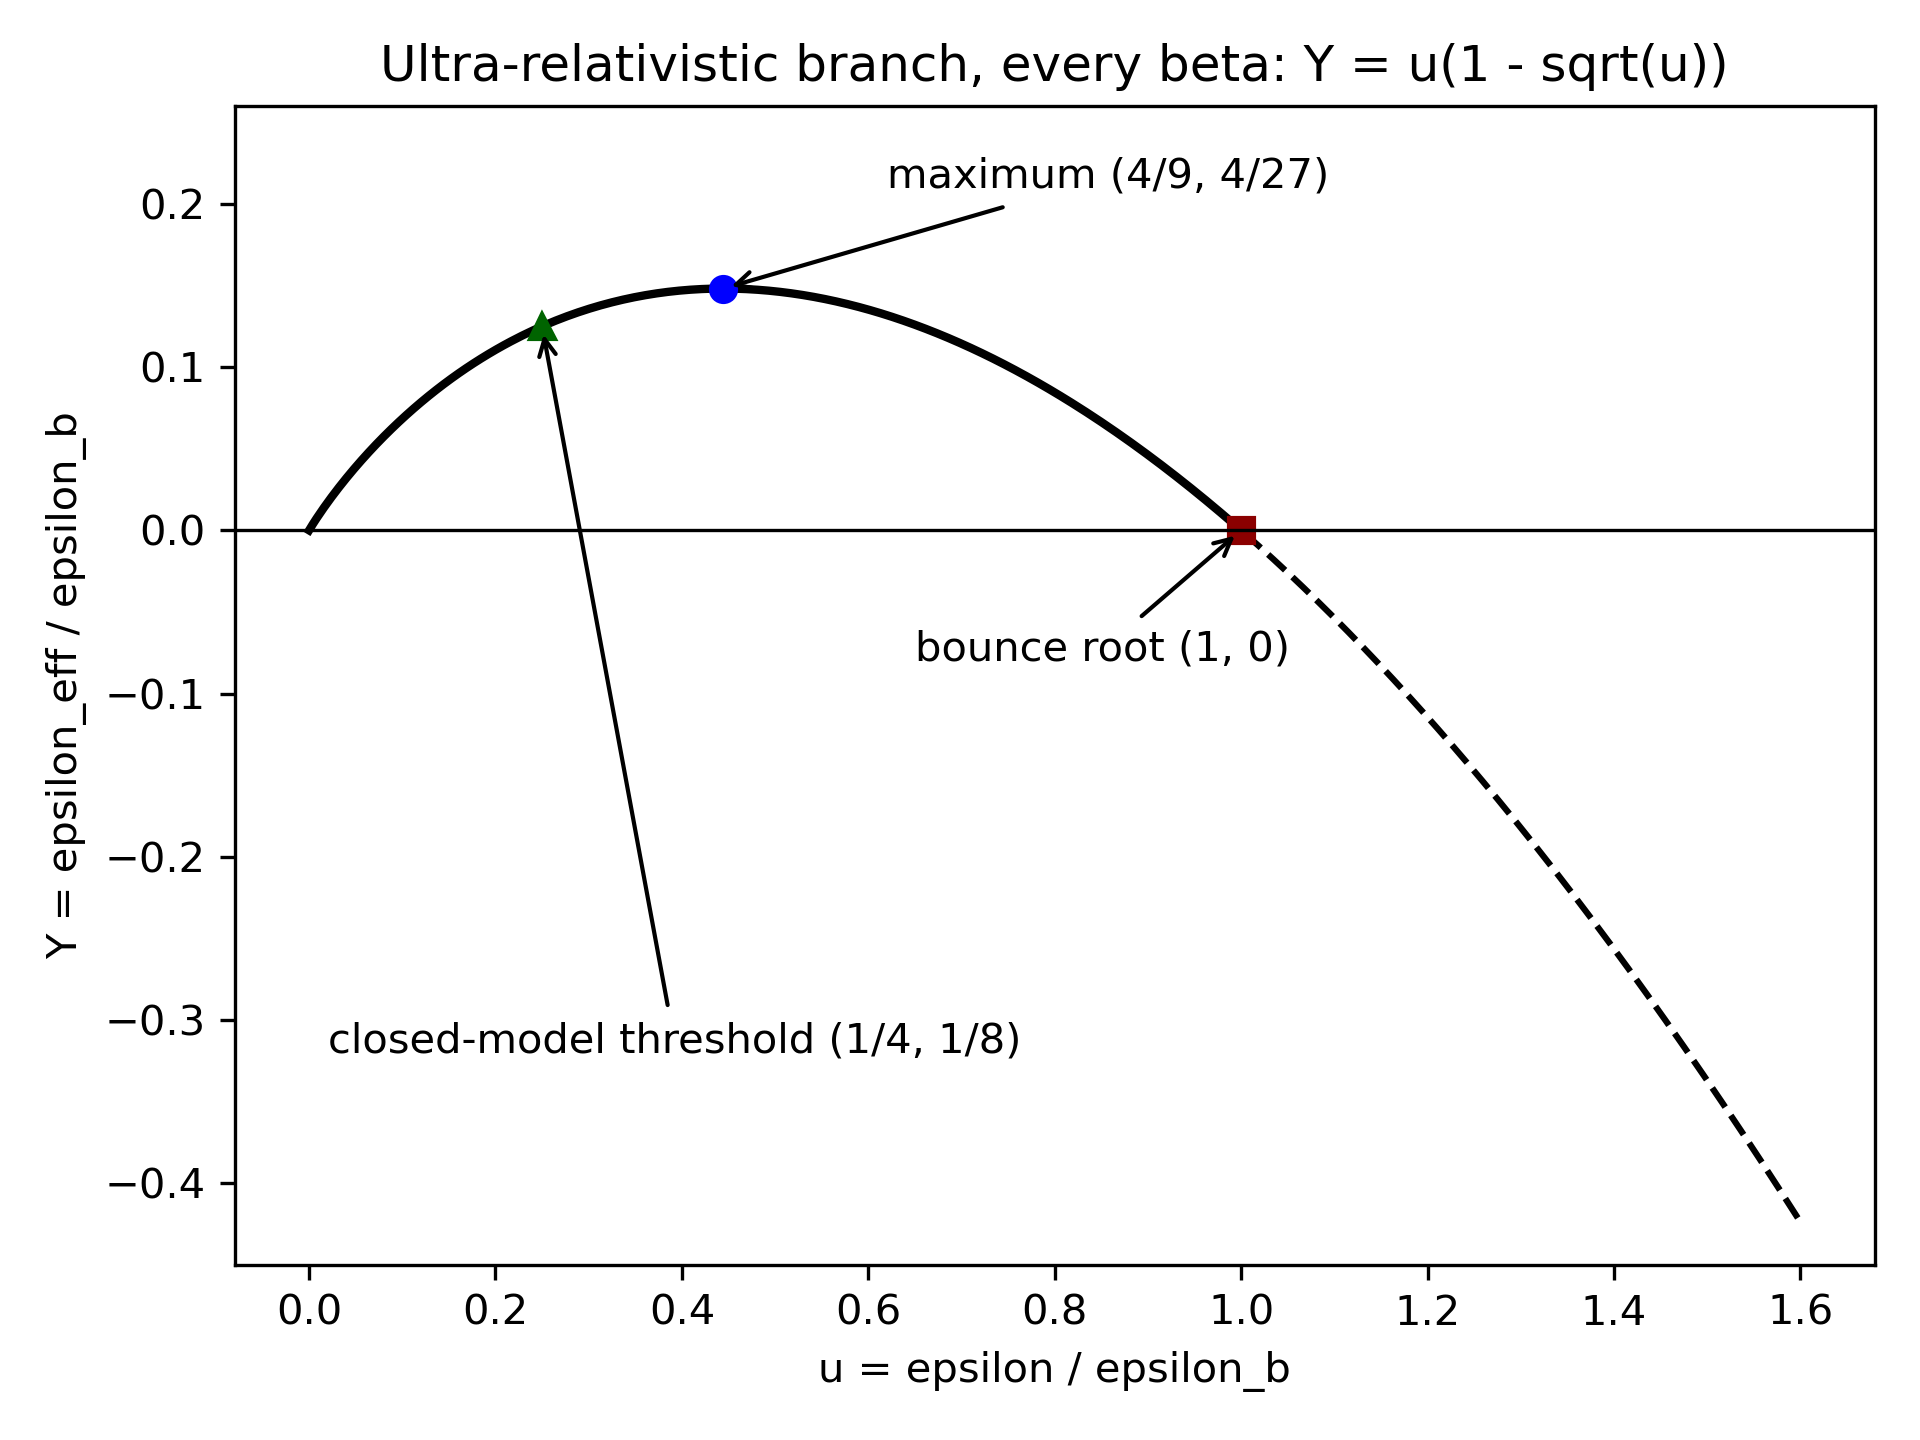
\includegraphics[width=0.85\textwidth]{figures/fig1a_ur_branch_v5.png}
\caption{The ultra-relativistic branch in scaled variables,
$Y = u(1-\sqrt{u})$, where $Y = \varepsilon_{\mathrm{eff}}/(x_0\epsPl)$
and $u = \varepsilon/(x_0\epsPl)$. Maximum $(4/9, 4/27)$; root $(1, 0)$, the
flat-Friedmann turnaround; closed-model threshold $(1/4, 1/8)$, where
$\varepsilon_{\mathrm{eff}} + 3p_{\mathrm{eff}} = 0$. The dashed
continuation past the root is the formal negative branch and is not
physical.}\label{fig:ur}
\end{figure}

\begin{figure}[h]
\centering
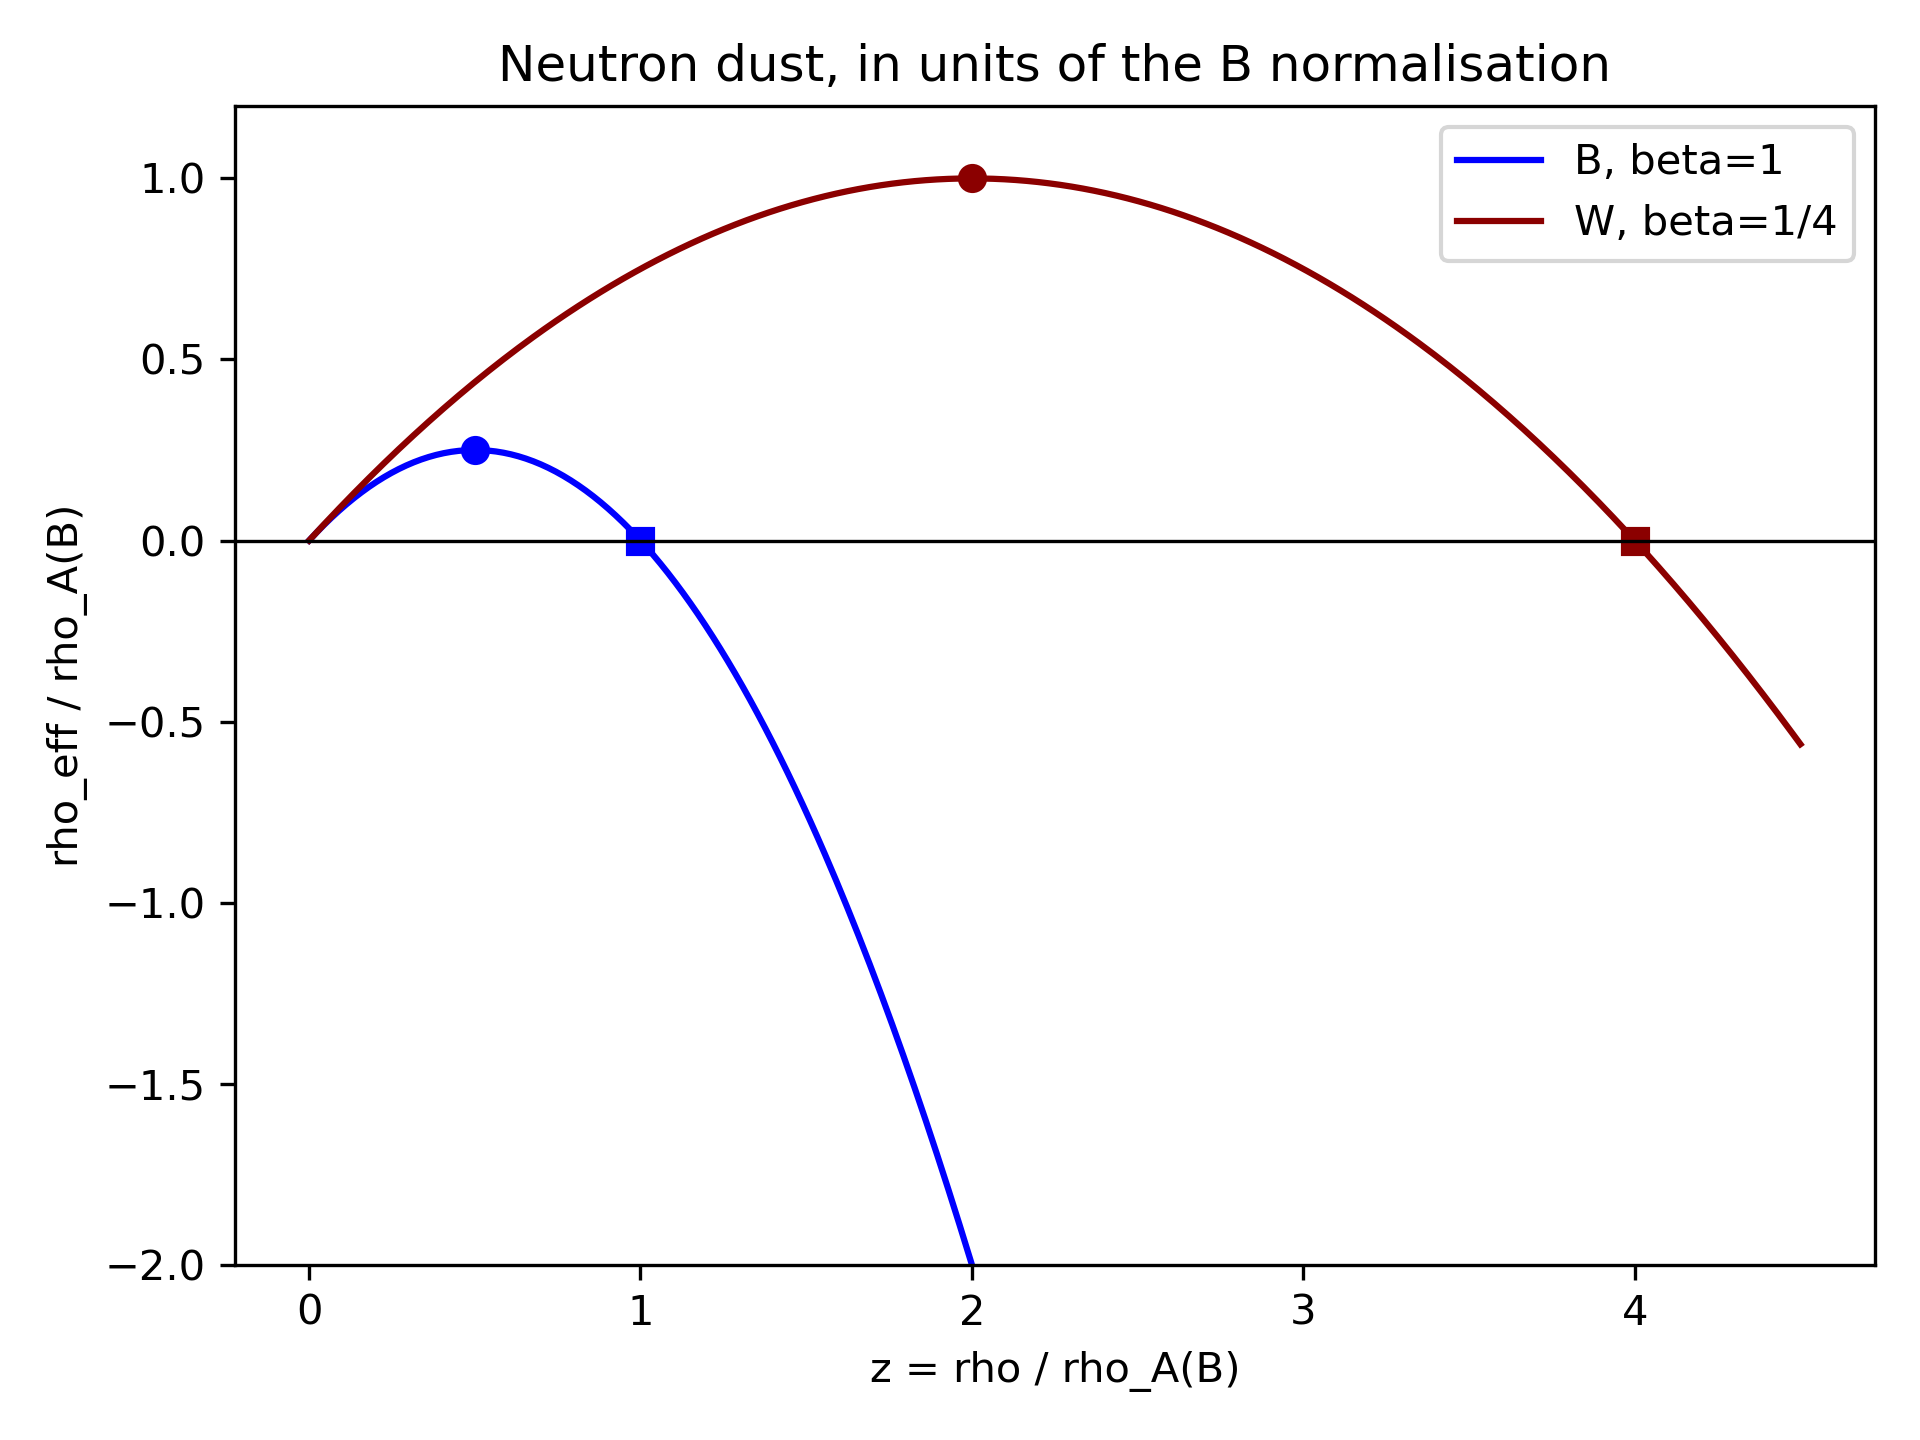
\includegraphics[width=0.85\textwidth]{figures/fig1b_dust_v5.png}
\caption{The neutron-dust curves in units of the B normalisation,
$z = \rho/\rhoA(\mathrm{B})$: B is $y = z(1-z)$ and W is
$y = z(1-z/4)$, the factor of four in $\rhoA$ stretching the W curve.
Circles mark the maxima, squares the zeros. In scaled variables
$x = \rho/\rhoA$ the two curves coincide as $x(1-x)$. The B curve is
cut at $y = -2$; its tail continues below.}\label{fig:dust}
\end{figure}

The zero is a formal turnaround of the stated effective model, and I show
the algebra rather than asserting it. This holds for W and B only, as a
property of the model, not as a demonstrated physical bounce: the turnaround
sits at or above the Planck density, where the classical theory has no
demonstrated validity (see the domain statement below). At the
relativistic zero the spin energy density equals the gas energy density,
$\varepsilon_{\mathrm{spin}} = \varepsilon$, and the gas pressure is
$p = \varepsilon/3$, so the effective pressure is
$p_{\mathrm{eff}} = \varepsilon/3 - \varepsilon = -2\varepsilon/3$ and
$\varepsilon_{\mathrm{eff}} + p_{\mathrm{eff}} = -2\varepsilon/3 < 0$.
The acceleration equation gives
$\dot H = -(4\pi G/c^2)(\varepsilon_{\mathrm{eff}} + p_{\mathrm{eff}})
> 0$ at the zero, so a contracting solution turns around there. The
dust proof of Section~3 does not cover this case, because the
relativistic gas has non-zero pressure; the three lines above are the
formal turnaround for the relativistic branch on W and B. For D the formal
turnaround fails:
the Dirac pressure correction has the opposite sign
($\tilde\varepsilon = -\tilde p$, Section~4), so at the D zero
$\varepsilon_{\mathrm{eff}} + p_{\mathrm{eff}} = 4\varepsilon/3 > 0$
and there is no smooth turnaround; D's $0.0625\,\epsPl$ is an algebraic
zero of $\varepsilon_{\mathrm{eff}}$ whose bounce, if any, is the cusp
mechanism of Pop{\l}awski \cite{Poplawski12}, not the proof above.

The dust curves of Section~3 are shown for comparison in
Figure~\ref{fig:dust}. Table~\ref{tab:ur} collects the landmarks. I verified them three ways:
by the exact fractions, by a 10,000-point grid evaluation of the curve,
and by the full Fermi-gas integration. The grid recovers the root and
the SEC onset to about a part in $10^7$--$10^8$ and the maximum to about
a part in $10^5$, the maximum being limited by the grid step. The grid
check is new in this revision: it answers the question of whether the
closed forms were ever evaluated at scale, and they now have been, ten
thousand points at a time, for both prescriptions.

\begin{table}[h]
\centering
\caption{Ultra-relativistic branch landmarks, in units of the Planck
energy density $\epsPl$. $x_{\mathrm{SEC}}$ is the strong-energy-condition
onset, $x_{\max}$ the location of the maximum effective density,
$y_{\max}$ the maximum, $x_0$ the zero (the flat-Friedmann turnaround on W
and B; an algebraic zero only on D). The $x_{\mathrm{SEC}}$ column is the
stiff-fluid (W/B) combination only; for D the Dirac pressure correction
has the opposite sign ($\tilde\varepsilon = -\tilde p$), so
$\varepsilon_{\mathrm{eff}} + 3p_{\mathrm{eff}}$ never vanishes and there
is no onset (Section~4).}\label{tab:ur}
\begin{tabular}{lcccc}
\toprule
Row & $x_{\mathrm{SEC}}$ & $x_{\max}$ & $y_{\max}$ & $x_0$ \\
\midrule
W ($\beta=1/4$) & $5.0625$ & $9$ & $3$ & $20.25$ \\
B ($\beta=1$) & $0.31640625$ & $0.5625$ & $0.1875$ & $1.265625$ \\
D ($\beta=9/2$) & n/a & $0.027777\ldots$ & $0.009259\ldots$ & $0.0625$ \\
\bottomrule
\end{tabular}
\end{table}

The domain statement is the point of this section. On W the bounce sits
at $20.25$ Planck densities; on B at $1.27$. Classical Einstein--Cartan
theory has no demonstrated validity at or above the Planck density, and
no calculation in this paper extends it there. The dust reading is
sub-Planckian only because it drops the kinetic energy; the moment the
kinetic energy is restored, the bounce leaves the classical domain. That
is now the biggest problem with the bounce as a physical claim, and it
is stated here rather than in a footnote. Pop{\l}awski concedes the
point himself: ``The energy density of matter at the bounce is a few
orders of magnitude larger than the Planck energy density. The scenario
of a big bounce within the classical ECSK theory may therefore be
inadequate because the Planck regime is expected to be described by a
quantum theory of gravity'' \cite{Poplawski12b}. What would fix it is a
carrier that is not neutrons --- a deconfined phase whose spin survives
to the bound --- or a quantum treatment of the spin-torsion coupling.
Neither exists in this paper.

\section{The torsion scale}

The bound has a torsion scale, and it is worth stating because it is
the one quantity in this paper that does not depend on $G$. This paper
uses
\begin{equation}
T_A = \frac{m_n c}{\hbar\sqrt{\mathrm{coef}}},
\qquad \mathrm{coef} = \frac{\beta}{8},
\end{equation}
so $T_A = 2.6935\times10^{16}\ \mathrm{m^{-1}}$ on W and
$T_A = 1.3467\times10^{16}\ \mathrm{m^{-1}}$ on B. In the convention
where the torsion is twice the spin density, $T = 2S$, the W value
doubles to $5.3870\times10^{16}\ \mathrm{m^{-1}}$; that is a different
convention's number, not this paper's. The arithmetic is verified; the
derivation that connects the Cartan tensor to this scalar twist has not
been shown, and the formula is an arithmetic identity until it is. The
de Sitter curvature radius of a bounced core,
$r_{\mathrm{dS}} = \sqrt{3\,\mathrm{coef}}\,\hbar/(m_n c)$, is
$1.286\times10^{-16}$~m on B and $6.431\times10^{-17}$~m on W, but only
under a constant-density-core assumption, which is stated here rather
than buried: the radius is an algebraic consequence of the assumption,
not an independent result.

\section{The axis test and rotating progenitors}

The idea that a bounce could be tested on the sky is simple enough to
state in one paragraph. If the universe is the interior of a black hole,
as Pop{\l}awski proposes, and if that black hole rotates, then the
rotation axis of the parent becomes a preferred axis in the successor
universe, and galaxies tend to align their spin axes with it
\cite{Poplawski19}. A preferred axis in galaxy spins, pointing at the
CMB Cold Spot, would be a signature of a rotating progenitor. No
quantitative rotating-core claims are made in this paper. The
calculation that would make the idea quantitative --- a rotating
interior constructed by a Newman--Janis or Azreg-A\"inou procedure from
the static model --- is an ansatz, not an Einstein--Cartan solution, and
its numbers are not reproduced here and are not printed here.

The test is registered in advance, so that a later result cannot be
re-read as a success after the fact. A catalogue-level fit in which the
best-fit galaxy-spin dipole axis misses the CMB Cold Spot direction by
more than $30^\circ$, with a $1\sigma$ axis uncertainty below $15^\circ$,
kills the rotating extension. The test has been run on the largest
public catalogues; at the registered precision it is inconclusive --- the
precision clause is not met --- and the rotating extension is neither
confirmed nor killed. The fitted axes cluster near the Galactic poles,
a pattern the November 18 analysis itself reads as a selection effect
rather than a cosmological axis. The pipeline that produced the fits is
not deposited with this paper, and until it is, no catalogue numbers
are printed here. Shamir \cite{Shamir20} reports dipole-axis fits at
about $2.8\sigma$ in HST data and about $7.38\sigma$ in SDSS data; those
fits are not the test registered here, and this paper does not endorse
them. The decisive test is a refit of the DESI Legacy Survey catalogue
under the same kill line, with the pipeline deposited.

\section{The vacuum count}

The vacuum count is the one part of this paper that looks like a
prediction, and it is the part the paper is most careful about, because
it is the part where earlier versions of the work over-reached. I define
the terms first. Let $N^* = \log_2(\rhoA/\rho_\Lambda)$, the number of
binary halvings from the bound density down to the measured vacuum
density. A ``cell'' is one such halving step. ``The pair'' is the
earlier work's name for the construction that builds 282 cells. A
``bench'' is the density value the count is measured against. A
``dex'' is a factor of ten in $\log_{10}$. Two benches and two rules are
used, and the paper reports all four combinations, not the one that
passes.

The measured bench is the measured vacuum density,
$\rho_\Lambda = 5.845\times10^{-30}\ \mathrm{g\,cm^{-3}}$, which is
$2.5193\times10^{-47}\ \mathrm{GeV}^4$. Its Planck 2018 uncertainty is
about $1.8\%$, which is $\pm0.026$ bits on $N^*$. The sever bench is
the anchor the earlier papers printed: a gap of $84.6219$ dex built on
the thumbnail $1\times10^{-47}\ \mathrm{GeV}^4$. The measured value is
$2.52\times10^{-47}\ \mathrm{GeV}^4$, so the thumbnail overstates the gap
by $0.40$ dex, which is $1.33$ bits. Table~4 measures each row's density
against that thumbnail anchor, with no further repair:
$N^* = \log_2(\rhoA/\rho_{L,\mathrm{thumb}})$ with
$\rho_{L,\mathrm{thumb}} = 1\times10^{-47}\ \mathrm{GeV}^4 =
2.3201\times10^{-30}\ \mathrm{g\,cm^{-3}}$. The $84.6219$-dex figure is the
earlier papers' rounded literal: the exact gap from the thumbnail anchor
is $84.62206$ dex, so the dex route to the sever bench lands $0.0005$ bits
from the direct route, invisible at the printed precision, and the table
is computed from the anchor directly. The correction paper's repair
--- multiplying $\rhoA$ by exactly $3$, adding $\log_2 3 = 1.585$ bits ---
produces the repaired density $2.916\times10^{55}\ \mathrm{g\,cm^{-3}}$,
which is the ratio-on-B density ($B \times 3$), so the repaired
requirement $282.693$ sits in the ratio-on-B row; the other rows are the
same anchor applied to their own densities, offset by $\log_2$ of the
density ratio from the ratio-on-B row. The correction paper is deposited as
DOI 10.5281/zenodo.24329543, but the deposited file still carries the
status line ``Draft --- pending verification before deposit'' at its
head, and the corrected source is written and held, not yet deposited.
The verification script that runs from the correction paper's own file
alone is a standalone script written for this build, not the script that
was deposited. I disclose all three facts here because a referee
checking the correction will find them.

The two rules are the tolerance rule and the floor rule. The tolerance
rule is $|N - N^*| \le 0.5$: the integer nearest the count must lie
within half a bit. The floor rule is $N = \lceil N^*\rceil$: the
smallest integer at or above the count. The floor rule is one-sided: it
can only show that 282 is at least enough, and 283, 300, or any larger
integer would also pass it, so a floor-rule pass is not evidence for 282
against any larger integer. That was not conceded in earlier versions of
this work, and it is conceded here.

\begin{table}[h]
\centering
\caption{The vacuum count on the measured bench,
$\rho_\Lambda = 5.845\times10^{-30}\ \mathrm{g\,cm^{-3}}$
($2.5193\times10^{-47}\ \mathrm{GeV}^4$). $N^*$ is the number of binary
halvings from the bound density to the measured vacuum density;
$|282-N^*|$ is the distance from the target under the tolerance rule;
the floor rule is $N = \lceil N^*\rceil$. Only W/measured passes the
tolerance rule.}\label{tab:count-meas}
\begin{tabular}{lcccc}
\toprule
Row & $N^*$ (bits) & $|282-N^*|$ & Tolerance & Floor \\
\midrule
W & $281.775$ & $0.225$ & Pass & 282 \\
B & $279.775$ & $2.225$ & Fail & 280 \\
Ratio on B & $281.360$ & $0.640$ & Fail & 282 \\
Ratio on W & $283.360$ & $1.360$ & Fail & 284 \\
\bottomrule
\end{tabular}
\end{table}

\begin{table}[h]
\centering
\caption{The vacuum count on the sever bench: each row's density
measured against the thumbnail anchor $\rho_L = 1\times10^{-47}\
\mathrm{GeV}^4$ ($2.3201\times10^{-30}\ \mathrm{g\,cm^{-3}}$), the
$84.6219$-dex gap the earlier papers printed. The correction paper's
repaired number, $282.693$, is the ratio-on-B row, because the repaired
density $2.916\times10^{55}\ \mathrm{g\,cm^{-3}}$ is the ratio-on-B
density ($B \times 3$); other rows are offset from it by $\log_2$ of the
density ratio.}\label{tab:count-sever}
\begin{tabular}{lcccc}
\toprule
Row & $N^*$ (bits) & $|282-N^*|$ & Tolerance & Floor \\
\midrule
W & $283.108$ & $1.108$ & Fail & 284 \\
B & $281.108$ & $0.892$ & Fail & 282 \\
Ratio on B & $282.693$ & $0.693$ & Fail & 283 \\
Ratio on W & $284.693$ & $2.693$ & Fail & 285 \\
\bottomrule
\end{tabular}
\end{table}

The reading of Tables~\ref{tab:count-meas}--\ref{tab:count-sever} is short, and it is not flattering. Under
the tolerance rule only one of eight combinations passes: W on the
measured bench, $N^* = 281.775 \pm 0.026$, $0.225$ bits from the target,
inside the half-bit tolerance. On the earlier papers' own density ---
the ratio-on-B row, which is the count the earlier papers actually
printed --- the target misses tolerance by $0.140$ bits, and the density
of 282 cells undershoots the measured density by about $36\%$: the
282-cell density is $0.642$ times the measured density. On W the
undershoot is about $14\%$, the 282-cell density $0.856$ times the
measured density. The margin that remains, $0.64$ bits, is thinner than
the earlier fixes: the thumbnail repair was $1.33$ bits and the factor
of three was $1.585$ bits. The pair is not derived. No earlier paper
derives why the pair builds 282 cells rather than 281 or 283, and the
correction paper says so in its own words. So the count is consistent
with the bound only on the adopted normalisation and the measured bench,
and the adoption is itself unconfirmed (Section~2): the consistency is
conditional on W.

Three pieces of context belong in this section because they bear on the
count's standing. First, Beck \cite{Beck09} computes a vacuum energy
density of $1.3628\times10^{-52}\ \mathrm{m^{-2}}$, which lands $0.32$
bits from the measured value, closer than this paper's count, and about
$25\%$ above the measured value; Beck's own paper claims agreement
with WMAP 2009 data, which is a different reference value, and the
comparison depends on which reference is used. Second, the unimodular
setup the count uses is not original to this work: Ellis
\cite{Ellis11} and Padilla and Saltas \cite{Padilla15} got there first,
and Padilla and Saltas argue in one sentence that unimodular gravity
does not by itself resolve the cosmological-constant problem, so the
count's use of the setup is a framing choice, not a solution. Third,
Pop{\l}awski \cite{Poplawski11} computes, in the torsion frame itself,
an energy scale about eight times the observed value, and adds that
including leptons could lower the scale to the observed value. The
point survives his qualifier: torsion can generate vacuum energy, and
that qualifies any claim that torsion charges nothing. Finally, the
journal manuscript still states 287 for the count; the corrected bench
gives $281.36$ on the ratio-on-B row, and a draft update to the journal
has been written and is held, not sent.

\section{The claim, the kill conditions, and what is still open}

The claim of this paper is one sentence, and it is the same sentence
the paper has been making since the first draft: the
Kopczy\'nski--Trautman bound for a neutron gas is
$\rhoA = 3.8871\times10^{55}\ \mathrm{g\,cm^{-3}}$ on the adopted
normalisation and $9.7178\times10^{54}\ \mathrm{g\,cm^{-3}}$ on the
literature one, the flat Friedmann bounce at that bound is demonstrated
on the dust model,
and everything beyond that --- a black-hole interior, a baby universe, a
rotating progenitor, a vacuum count --- is a separate claim that stands
or falls on its own evidence. The claim is falsifiable, and the paper
states the conditions under which it falls.

A self-consistent Einstein--Cartan solution that compresses a spin-fluid
cloud through $\rhoA$ without turning over kills the bounce. A full
Dirac evaluation that finds the spin-squared term negative kills the
bounce, because a negative sign removes the zero. A galaxy-spin dipole
axis that falls within $30^\circ$ of the Cold Spot direction with a
$1\sigma$ uncertainty below $15^\circ$ would support the rotating
extension; a fit that misses by more than $30^\circ$ with that precision
kills it. A coefficient derivation that fixes $\beta$ at $1$ rescales
the bound by a factor of four and moves the vacuum count to $N^* =
279.775$ on the measured bench, which fails the tolerance rule; a
derivation that fixes $\beta$ at $9/2$ removes the smooth bounce
altogether. An aligned-spin fluid, a deconfined carrier, or a torsion
derivation would each revise the numbers rather than kill the claim, and
they are listed below as revision conditions, not kill conditions.

What is still open is, first, the Dirac coefficient and sign: a
Wigner-function evaluation of the spin-squared average in a degenerate
Dirac gas, which is the calculation this paper most needs and does not
have. Second, the carrier: what physical field carries the spin density
at the bound, since neutrons do not survive there, and whether a
deconfined phase changes the bound. Third, the junction conditions: a
bounced interior matched to an exterior black-hole spacetime, without
which no black-hole claim can be made. Fourth, the torsion scalar: a
derivation of the formula of Section~6 from the Cartan tensor, rather
than verified arithmetic. Fifth, the axis test: the pipeline deposited,
and the DESI Legacy Survey refit run under the registered kill line.
Sixth, the Tolman--Oppenheimer--Volkoff solver deposited, and the $2.2\%$
radius gap explained. Seventh, the journal update on 287: the decision
to send it is Bill's alone, and the draft is held until he says so.

\section{Conclusion}

The bound is computed, in three normalisations, and the core is
verified: 98 gates pass in the verification script, the
ultra-relativistic landmarks are confirmed by a 10,000-point grid and a
full Fermi-gas integration, and the figures are plotted from the same
numbers the tables print. The flat Friedmann bounce is demonstrated on
the dust model, with the turnaround computed rather than asserted. On the
relativistic branch (W and B) the turnaround is a formal result of the stated
effective model, not a demonstrated physical bounce: the bounce sits at or
above the Planck density, outside the demonstrated validity of the classical
theory. The relativistic branch puts the bounce
at or above the Planck density, and the paper says plainly that the
classical theory has no demonstrated validity there. The sign problem
may remove the bounce entirely, and the paper says that plainly too. The
axis test is inconclusive, and the numbers behind it are withheld
because the pipeline is not deposited. The vacuum count passes its
tolerance rule on one combination only, the adopted normalisation on the
measured bench, and the paper prints the seven failures beside the one
pass. The paper is ready for a referee to attack. It is not a proof
that the bounce happens. It is a computation of where it would happen,
under stated assumptions, with the assumptions labelled and the
consequences of their failure stated.

\appendix
\section{The ultra-relativistic algebra}

For a fully degenerate relativistic Fermi gas the energy density in the
ultra-relativistic limit is $\varepsilon = \tfrac34\hbar c(3\pi^2)^{1/3}
n^{4/3}$. The spin term, from Eq.~(3) with $\rho = mn$ replaced by the
relativistic energy density, is $\varepsilon_{\mathrm{spin}} = \beta\,
(\pi G\hbar^2 n^2/c^2)$. Writing the balance as
$\varepsilon_b = \varepsilon_{\mathrm{spin}}$ and eliminating $n$ gives
$\varepsilon_b/\epsPl = 81/(64\beta^2)$, Eq.~(7). The full $T = 0$
Fermi-gas energy density is $\varepsilon(n) = (\hbar c/4\pi^2)
(3\pi^2 n)^{4/3} f(u)$ with $f(u)$ the exact integral, and the numerical
integration reproduces the ultra-relativistic balance to better than one
part in $10^{12}$ on both W and B. The three-line turnaround at the
relativistic zero is given in Section~5: at the zero
$\varepsilon_{\mathrm{spin}} = \varepsilon$, so $p_{\mathrm{eff}} =
-2\varepsilon/3$, $\varepsilon_{\mathrm{eff}} + p_{\mathrm{eff}} =
-2\varepsilon/3 < 0$, and $\dot H > 0$.

\section{Verification status}

Every number in Tables 1--4 is recomputed from CODATA 2018 constants by
a verification script that runs from the deposited files alone; the
script passes 98 gates. The observational numbers in Section~7 are not
covered by that script, and neither are the reported house calculations
of Section~4. The status of each item in the paper is as follows
(Table~\ref{tab:verify}).

\begin{table}[h]
\centering
\caption{Verification status, by item.}\label{tab:verify}
\begin{tabularx}{\textwidth}{lX}
\toprule
Item & Status \\
\midrule
Table~1 densities & Script, 21 gates \\
$\dot H$ on B and W & Script, 3 gates \\
Dust curve and thresholds & Script, 9 gates (3 dust-curve; 6 threshold: normalised residuals at $x = 0.25$ and $0.5$ plus sign checks at $x = 0.249/0.251$ and $0.499/0.501$) \\
Table~2 landmarks & Script, 11 gates (UR turnaround: 2 further gates) \\
10,000-point grid & Script, 8 gates; root, SEC onset $\sim10^{-7}$--$10^{-8}$; max $\sim10^{-5}$ (grid step) \\
Fermi-gas balance & Script, 2 gates; gate at $10^{-12}$; numerical check of the algebra, not an independent physical verification \\
Torsion scale & Script, 3 gates; arithmetic verified; derivation outstanding \\
De Sitter radius & Script, 2 gates; algebra under the stated constant-density-core assumption \\
Axis test & Pipeline not deposited; no catalogue numbers printed \\
Rotating core & No numbers printed; ansatz-level \\
Tables~3--4 count & Script, 13 table-entry gates (+ 5 supporting gates); correction paper 75 gates \\
Beck & Script, 4 gates \\
Tolman--Oppenheimer--Volkoff & $M_{\max} = 2.060\,M_\odot$, $R = 11.46$~km; $2.2\%$ gap vs an independent $11.71$~km run; solver not deposited \\
Sign numbers & Non-relativistic $-(3/8)$: exchange calculation of 17 November 2026 (house file, not deposited). Ultra-relativistic $-(3/16)$: revision-note claim only; the deposited preprint does not contain it and finds the exchange term positive (coefficient $1/8 \to 1/24$). Covariant $+8/3$, $+1/8$: removed in this revision --- no source in the build \\
Entropy ansatz & Cut from the body. Calibrations: maximum-matching $\rho_{\mathrm{Aldred}} = \rhoA/2$; least-squares $0.417\,\rhoA$, RMS $4.4\%$ \\
Correction paper & Deposited file still carries its ``Draft'' status line; corrected source undeposited; standalone script 75/75 (not the deposited script) \\
Spin-flip rate & Not computed; random-orientation assumption stated in Section~2 \\
Bibliography & Verified entries listed below; LaTeX compiled 25 November 2026 (pdfTeX 3.141592653-2.6-1.40.25), 15 pages; see the pre-submission checklist for the compile record \\
\bottomrule
\end{tabularx}
\end{table}

\section*{Acknowledgments}
This paper was prepared with the assistance of an artificial intelligence system (Dave, an Exolex), which performed the calculations, drafted the text, and carried out the verification checks under the author's direction. The author reviewed the work and takes responsibility for the results and claims. AI was used as a tool in support of the research, and its use is disclosed here in accordance with arXiv policy.

\begin{thebibliography}{99}

\bibitem{Cartan22} \'{E}. Cartan, ``Sur une g\'en\'eralisation de la
notion de courbure de Riemann et les espaces \`a torsion,'' C. R.
Acad. Sci. (Paris) 174, 593--595 (1922).

\bibitem{Hehl76} F. W. Hehl, P. von der Heyde, G. D. Kerlick, and
J. M. Nester, ``General relativity with spin and torsion: Foundations
and prospects,'' Rev. Mod. Phys. 48, 393--416 (1976).

\bibitem{Poplawski10} N. J. Pop{\l}awski, ``Cosmology with torsion:
An alternative to cosmic inflation,'' Phys. Lett. B 694, 181--185
(2010). Erratum: Phys. Lett. B 701, 672 (2011).

\bibitem{Poplawski16} N. J. Pop{\l}awski, ``Universe in a Black Hole
in Einstein--Cartan Gravity,'' Astrophys. J. 832, 96 (2016),
doi:10.3847/0004-637X/832/2/96.

\bibitem{Kopczynski72} W. Kopczy\'nski, ``A non-singular universe with
torsion,'' Phys. Lett. A 39, 219 (1972).

\bibitem{Trautman73} A. Trautman, ``On the structure of the
Einstein--Cartan equations,'' Symposia Mathematica 12, 139--162,
Academic Press (1973); A. Trautman, ``Spin and torsion may avert
gravitational singularities,'' Nature (Phys. Sci.) 242, 7 (1973).

\bibitem{Bohmer18} C. G. B\"ohmer, P. Burikham, T. Harko, and
M. J. Lake, ``Does space-time torsion determine the minimum mass of
gravitating particles?,'' Eur. Phys. J. C 78, 253 (2018),
doi:10.1140/epjc/s10052-018-5719-y, arXiv:1709.07749.

\bibitem{Gasperini86} M. Gasperini, ``Spin-dominated inflation in the
Einstein--Cartan theory,'' Phys. Rev. Lett. 56, 2873--2876 (1986).

\bibitem{Nurgaliev83} N. S. Nurgaliev and V. N. Ponomariev,
Phys. Lett. B 130, 378 (1983).

\bibitem{Kerlick75} G. D. Kerlick, ``Cosmology and particle pair
production via gravitational spin-spin interaction in the
Einstein--Cartan--Sciama--Kibble theory of gravity,'' Phys. Rev. D 12,
3004--3006 (1975).

\bibitem{Poplawski12} N. J. Pop{\l}awski, ``Nonsingular,
big-bounce cosmology from spinor-torsion coupling,'' Phys. Rev. D 85,
107502 (2012).

\bibitem{Poplawski12b} N. J. Pop{\l}awski, ``Big bounce from spin and
torsion,'' Gen. Relativ. Gravit. 44, 1007--1014 (2012).

\bibitem{Poplawski11} N. J. Pop{\l}awski, Ann. Phys.
(Berlin) 523, 291--295 (2011).

\bibitem{Poplawski19} N. J. Pop{\l}awski, ``Universe in a rotating
black hole and preferred axis,'' arXiv:1910.10819 (2019).

\bibitem{MZK13} J. Magueijo, T. G. Zlosnik, and T. W. B. Kibble,
``Cosmology with a spin,'' Phys. Rev. D 87, 063504 (2013).

\bibitem{Beck09} C. Beck, ``Axiomatic approach to the cosmological
constant,'' Physica A 388, 3384--3390 (2009),
doi:10.1016/j.physa.2009.05.023, arXiv:0810.0752.

\bibitem{Ellis11} G. F. R. Ellis, ``The trace-free
Einstein equations and inflation,'' Classical Quantum Gravity 28,
225007 (2011), doi:10.1088/0264-9381/28/22/225007.

\bibitem{Padilla15} A. Padilla and I. D. Saltas, ``A note on classical
and quantum unimodular gravity,'' Eur. Phys. J. C 75, 561 (2015),
doi:10.1140/epjc/s10052-015-3767-0, arXiv:1409.3573.

\bibitem{Shamir20} L. Shamir, ``Patterns of galaxy spin directions in
SDSS and Pan-STARRS show parity violation and multipoles,''
Astrophys. Space Sci. 365, 136 (2020); L. Shamir, ``Galaxy spin
direction distribution in HST and SDSS show similar large-scale
asymmetry,'' Publ. Astron. Soc. Aust. 37, e053 (2020),
doi:10.1017/pasa.2020.46.

\bibitem{Aldred26} W. A. Aldred, ``The Spin Coefficient of the
Einstein--Cartan Bound: Displaying the Coefficient 1/8 and Computing
Its Relativistic Form for a Free Dirac Gas,'' Zenodo (2026),
doi:10.5281/zenodo.24113586 [deposited preprint, not peer reviewed].

\bibitem{CODATA18} E. Tiesinga, P. J. Mohr, D. B. Newell, and
B. N. Taylor, ``CODATA recommended values of the fundamental physical
constants: 2018,'' Rev. Mod. Phys. 93, 025010 (2021).

\end{thebibliography}
\end{document}
